
\lhead[\chaptername~\thechapter]{\rightmark}

\rhead[\leftmark]{}

\lfoot[\thepage]{}

\cfoot{}

\rfoot[]{\thepage}

\chapter{Methods}

In this chapter, methods used for performing the change point analysis
in this thesis are explained. It first starts by providing general
information about Markov chains. Later on, the simple Markov switching
model feature and model specification namely Markov switching autoregressive
model are discussed. Thereafter, three sections are devoted to methods
for estimating the values of parameters, predicting a state for a
new observation and selecting a suitable model for the datasets. Another
change-point method in a non-parametric approach is described. Finally,
the simulation technique  is explained.

\section{Markov chains\label{sec:Markov-chains}}

A Markov chain is a random process which has a property that is given
the current value, the future is independent of the past. A random
process $X$ contains random variables $X_{t}:\:t\in T$ indexed by
a set $T$. When $T=\{0,1,2,...\}$ the process is called a discrete-time
process, and when $T=[0,\infty)$ it is called a continuous-time process.
Let $X_{t}$ be a sequence of values from a state space $S$. The
process begins from one of these states and moves to another state.
The move between states is called a step. The process of Markov chains
is described here.
\begin{defn}
\citep[p.214]{grimmett2001probability} If a process $X$ satisfies
the Markov property, the process $X$ is a first order Markov chain

\[
P(X_{t}=s|X_{0}=x_{0},X_{1}=x_{1},...,X_{t-1}=x_{t-1})=P(X_{t}=s|X_{t-1}=x_{t-1})
\]

where $t\ge1$ and $s,x_{0},...,x_{t-1}\in S$
\end{defn}
If $X_{t}=i$ then the chain is in state $i$ or the chain is in the
$i$th state at the $t$th step. 

There are transitions between states which describe the distribution
of the next state given the current state. The evolution of changing
from $X_{t}=i$ to $X_{t}=j$ is defined by the transition probability
as $P(X_{t}=j|X_{t-1}=i)$. For Markov chains, it is frequently assumed
that these probabilities depend only on $i$ and $j$ and do not depend
on $t$.
\begin{defn}
\citep[p.214]{grimmett2001probability} The chain is time-homogeneous
if

\[
P(X_{t+1}=j|X_{t}=i)=P(X_{1}=j|X_{0}=i)
\]

for all $t,i,j$. The probability of the transition is independent
of $t$. A transition matrix $\mathbf{P}=(p_{ij})$ is a matrix of
transition probabilities 

\[
p_{ij}=P(X_{t}=j|X_{t-1}=i)
\]
\end{defn}
\begin{thm*}
\citep[p.215]{grimmett2001probability} The transition matrix $\mathbf{P}$
is a matrix that
\begin{itemize}
\item Each of the entries is a non-negative real number or $p_{ij}\ge0$
for all $i,j$
\item The sum of each row equal to one or $\sum_{j}p_{ij}=1$ for all $i$
\end{itemize}
\end{thm*}

\begin{defn}
\citep[p.220]{grimmett2001probability} State $i$ is called persistent
(or recurrent) if

\[
P(X_{t}=i\mathrm{\:for\,}\mathrm{some\,\mathrm{n}}\geq1|X_{0}=i)=1
\]
\end{defn}

Let $f_{ij}(n)=P(X_{1}\neq j,X_{2}\neq j,...,X_{t}\neq j|X_{0}=i)$
be the probability of visiting state $j$ first by starting from $i$,
takes place at $t$th step.

\begin{defn}
\citep[p.222]{grimmett2001probability} The mean recurrence time of
a state $i$ is defined as

\[
\mu_{i}=E(T_{i}|X_{0}=i)=\sum_{n}n\cdot f_{ii}(n)
\]

State $i$ is a non-null persistent (or positive recurrent) if $\mu_{i}$
is finite. Otherwise, the state $i$ is null persistent. 
\end{defn}

\begin{defn}
\citep[p.222]{grimmett2001probability} A state $i$ that has a period
$d(i)$ is defined as 

\[
d(i)=gcd\{n:\:p_{ii}(n)>0\}
\]

where $gcd$ is the greatest common divisor. If $d(i)=1$, then the
state is said to be aperiodic. Otherwise, the state is said to be
periodic. 
\end{defn}

\begin{defn}
\citep[p.222]{grimmett2001probability} A state is called ergodic
if it is non-null persistent and aperiodic.
\end{defn}

\begin{defn}
A chain is called irreducible if it is possible to go from every state
to every other states.
\end{defn}

\begin{thm*}
\citep{manning2008introduction} If there is a aperiodic finite state
space, an irreducible Markov chain is the same thing as ergodic Markov
chain. 
\end{thm*}

\section{Markov switching model}

A Markov switching model is a switching model where the shifting back
and forth between the states or regimes is controlled by a latent
Markov chain. The model structure consists of two stochastic processes
embedded in two levels of hierarchy. One process is an underlying
stochastic process that is not normally observable, but possible to
be observed through another stochastic process which generates the
sequence of observation \citep{rabiner1986introduction}. The time
that transition between state occurs is random. In addition, the state
transition are assumed to follow the Markov property that the future
state depends only on the current state. 

The Markov switching model is able to model more complex stochastic
processes and describe changes in the dynamic behavior. A general
structure of the model can be drawn graphically as shown in \ref{msm},
where $S_{t}$ and $y_{t}$ denote the state sequence and observation
sequence in the Markov process, respectively. The arrows from one
state to another state in the diagram implies a conditional dependency. 

\begin{figure}[H]
\begin{centering}
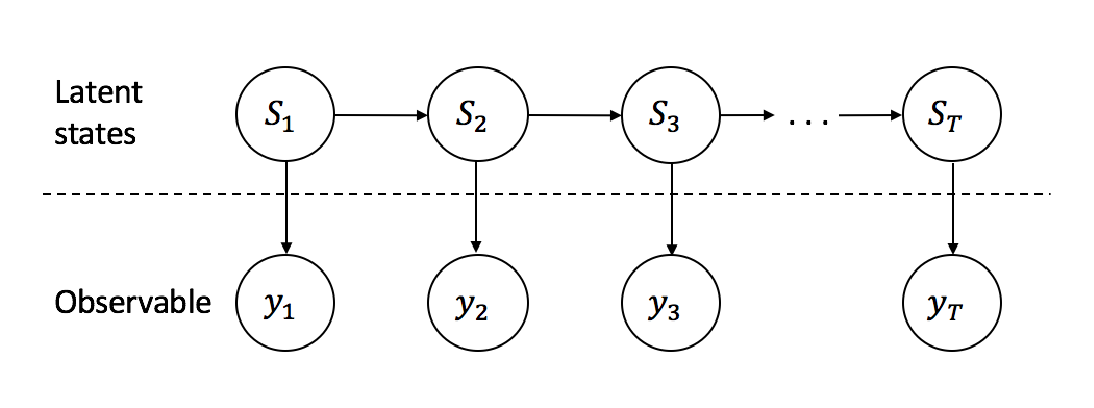
\includegraphics[scale=0.7]{picture/msm1}
\par\end{centering}
\caption{Model structure}
\label{msm}
\end{figure}

The process is given by \citep{hamilton1989new}

\begin{equation}
y_{t}=X_{t}\beta_{S_{t}}+\varepsilon_{t}\label{eq:general_mswm}
\end{equation}
where, 
\begin{labeling}{00.00.0000}
\item [{$y_{t}$}] is an observed value of the time series at time $t$
\item [{$X_{t}$}] is a design matrix, also known as model matrix, containing
values of predictor variables of the time series at time $t$
\item [{$\beta_{S_{t}}$}] are a column vector of coefficients in state
$S_{t}$, where $S_{t}\in\{1,...,k\}$ %
\begin{comment}
$1\leqslant i\leqslant k$ 
\end{comment}
\item [{$\varepsilon_{t}$}] follows a Normal distribution with zero mean
and variance given by $\sigma_{S_{t}}^{2}$ 
\end{labeling}
Equation \ref{eq:general_mswm} is the simplest form for the switching
model.%
\begin{comment}
where there are $k-1$ structural breaks in the model parameters.
\end{comment}
{} To aid understanding, the baseline model is assumed to have only
two states $(k=2)$ in this discussion. $S_{t}$ is a random variable
which is assumed that the value $S_{t}=1$ for $t=1,2,...,t_{0}$
and $S_{t}=2$ for $t=t_{0}+1,t_{0}+2,...,T$ where $t_{0}$ is a
known change point. 

The transition matrix $\mathbf{P}$ is an $2\mathrm{x}2$ matrix where
row $j$ column $i$ element is the transition probability $p_{ij}$.
A diagram showing a state-transition is shown in \ref{transition}.
Note that these probabilities are independent of $t$.

\begin{figure}[H]
\begin{centering}
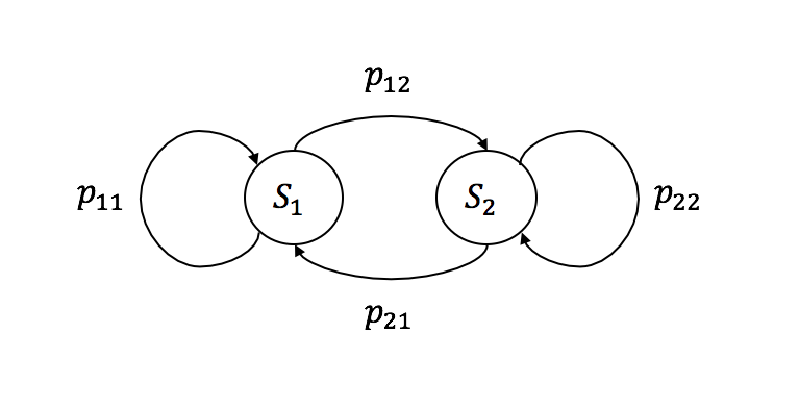
\includegraphics[scale=0.6]{picture/transition}
\par\end{centering}
\caption{State-transition diagram}
\label{transition}
\end{figure}

Since the whole process $S_{t}$ is unobserved, the initial state
where $t=0$ also needs to be specified. The probability which describes
the starting distribution over states is denoted by

\[
\pi_{i}=P(S_{0}=i)
\]

There are several options for computing the probability of the initial
state. One procedure is to commonly set $P(S_{0}=i)=0.5$. Alternatively,
the unconditional probability of $S_{t}$ 

\[
\pi_{1}=P(S_{0}=1)=\frac{1-p_{jj}}{2-p_{ii}-p_{jj}}
\]

can be used by presuming an ergodic Markov chain \citep{hamilton2005regime}.
\newline

A coefficient of a predictor variable in the Markov switching model
can have either different values in different state or a constant
value in all state. The variable which have the former behavior is
said to have a \emph{switching effect}. Likewise, the variable which
have the same coefficient in all states is a variable that does not
have a switching effect, or said to have a \emph{non-switching effect.}
\begin{comment}
The predictor variable which has a switching effect is called state-dependent.
Likewise, the predictor variable which has a non-switching effect
is called state-independent.
\end{comment}

A generalized form of Equation \ref{eq:general_mswm} can be defined
as \citep{perlin2015ms_regress}

\begin{comment}
\begin{equation}
y_{t}=\sum_{i=1}^{N_{s}}\beta_{i,S_{t}}X_{\text{i,}t}^{s}+\sum_{j=1}^{N_{ns}}\beta_{j,t}X_{j,t}^{ns}+\varepsilon_{t}
\end{equation}

$N_{s}$ is the number of switching coefficients in the model

$N_{ns}$ is the number of non-switching coefficients in the model
\end{comment}

\begin{equation}
y_{t}=X_{t}^{ns}\alpha_{t}+X_{t}^{s}\beta_{S_{t}}+\varepsilon_{t}
\end{equation}

where, 
\begin{labeling}{00.00.0000}
\item [{$X_{t}^{ns}$}] contains all predictor variables that have non-switching
effect of the time series at time $t$
\item [{$\alpha_{t}$}] are non-switching coefficients of the time series
at time $t$
\item [{$X_{t}^{s}$}] contains all predictor variables that have the switching
effect of the time series at time $t$
\item [{$\beta_{S_{t}}$}] are switching coefficients in state $S_{t}$,
where $S_{t}\in\{1,...,k\}$
\item [{$\varepsilon_{t}$}] follows a Normal distribution with zero mean
and variance given by $\sigma_{S_{t}}^{2}$ 
\end{labeling}

\subsection{Autoregressive (AR) model}

An autoregressive model is one type of time series models used to
describe a time-varying process. The model is flexible in handling
various kinds of time series patterns. The name autoregressive comes
from how the model performs a regression of the variable against its
own previous outputs \citep{cryer1986time}. The number of autoregressive
lags (i.e., the number of prior values used in the model%
\begin{comment}
 a time span between observations/ a later point in the data series
\end{comment}
) is denoted by $p$. 
\begin{defn}
An autoregressive model of order $p$ or AR(p) model can be written
as 

\[
y_{t}=c+\phi_{1}y_{t-1}+\phi_{2}y_{t-2}+...+\phi_{p}y_{t-p}+\varepsilon_{t}
\]
or

\[
y_{t}=c+\sum_{i=1}^{p}\phi_{i}y_{t-i}+\varepsilon_{t}
\]

where $c$ is a constant, $\phi_{i}$ are coefficients in the autoregression
and $\varepsilon_{t}$ is a Gaussian white noise with zero mean and
variance $\sigma^{2}$.
\end{defn}
If $p$ is equal to one, the model AR(1) is called the first order
autoregression process.

\subsection{Markov switching autoregressive model}

A Markov switching autoregressive model is an extension of a basic
Markov switching model where observations are drawn from an autoregression
process. The model relaxes the conditional independent assumption
by allowing an observation to depend on both past observation and
a current state \citep{shannon2009formulation}. Basically, this is
the combination between the Markov switching model and the autoregressive
model.
\begin{defn}
The first order Markov switching autoregressive model is 

\[
y_{t}=X_{t}\beta_{S_{t}}+\phi_{1,S_{t}}y_{t-1}+\varepsilon_{t}
\]

where $\phi_{1,S_{t}}$ is an autoregression coefficient of the observed
value at time $t-1$ in state $S_{t}$. $\varepsilon_{t}$ follows
a Normal distribution with zero mean and variance given by $\sigma_{S_{t}}^{2}$.
\end{defn}
The structure of the model is shown in \ref{msm-ar}. It can be clearly
seen that there is a dependency at the observation level.%
\begin{comment}
 and that observations are not independent from one another. 
\end{comment}

\begin{figure}[H]
\begin{centering}
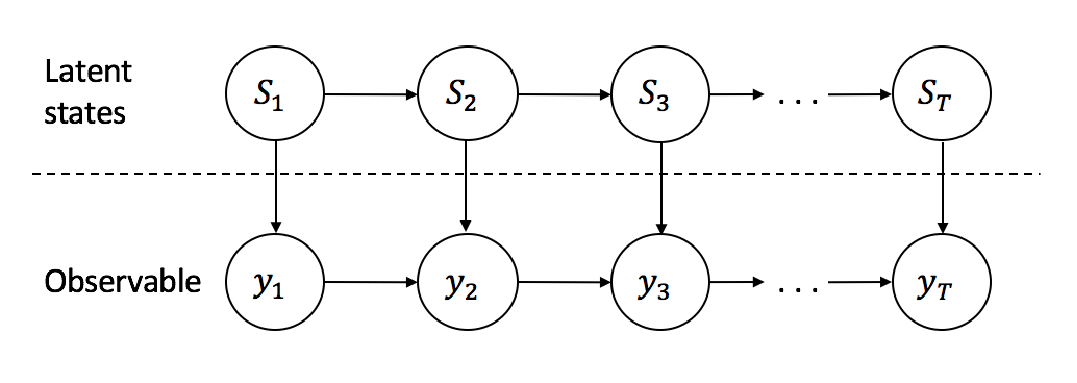
\includegraphics[scale=0.7]{picture/msm-ar1}
\par\end{centering}
\caption{Model structure of Markov switching AR(1)}
\label{msm-ar}
\end{figure}

Assuming two states $S_{t}=1$ or $2$, the set of parameters that
are necessary to describe the law of probability that governs $y_{t}$
are $\theta=\{\beta_{1},\beta_{2},\phi_{1,1},\phi_{1,2},\sigma_{1}^{2},\sigma_{2}^{2},\pi_{1},\pi_{2},p_{11},p_{22}\}$. 

\section{Parameter estimation}

There are various ways to estimate parameters of Markov switching
model. Methods which have been widely used are as follow: E-M algorithm
\citep{hamilton1990analysis,kim1994dynamic} used the maximum likelihood
criterion, Segmental K-means \citep{juang1990segmental} used K-means
algorithm and maximized the state-optimized likelihood criterion,
and Gibbs sampling \citep{kim1999state} used a Markov chain Monte
Carlo simulation method based on the Bayesian inference. 

In this thesis framework, the E-M algorithm is used in estimating
parameters as the algorithm gives an effective results, numerically
stable, and easy to implement. \citet{ryden2008versus} compared the
computational perspective between the E-M algorithm and the Gibbs
sampling in estimating parameters. In most cases, Gibbs sampling tended
to have less computational time than the E-M algorithm. However, the
study indicated that if the number of states was unknown, the E-M
algorithm would be simpler and quicker in computing the estimated
parameters for all candidate models. The E-M algorithm is briefly
described below. %
\begin{comment}
Summing up this case, we first remark that if one wants to compute
only the best model without any further information on how plausible
it is relative to other ones, then the simplest solution is using
EM to compute MLEs for all candidate models and then calculating and
comparing their BICs or some other penalized likelihood criterion.
\end{comment}


\subsection{The Expectation-Maximization algorithm}

E-M algorithm is originally designed to deal with the problem of incomplete
or missing values in data \citep{dempster1977maximum}. Nevertheless,
it could be implemented in Markov switching model since the unobserved
state $S_{t}$ can be viewed as missing data values. 

The set of parameters $\theta$ are estimated by an iterative two-step
procedure. In the first step, the algorithm starts with arbitrary
initial parameters, and then finds the expected values of the state
process from the given observations. In the second step of the iterative
procedure, a new maximum likelihood from the derived parameters in
the previous step is calculated. These two steps are repeated until
the maximum value of the likelihood function is reached or converged
\citep{janczura2012efficient}. The two steps are known as the E-step
and the M-step. \ref{em} illustrates the process of the E-M algorithm.

\begin{figure}[H]
\begin{centering}
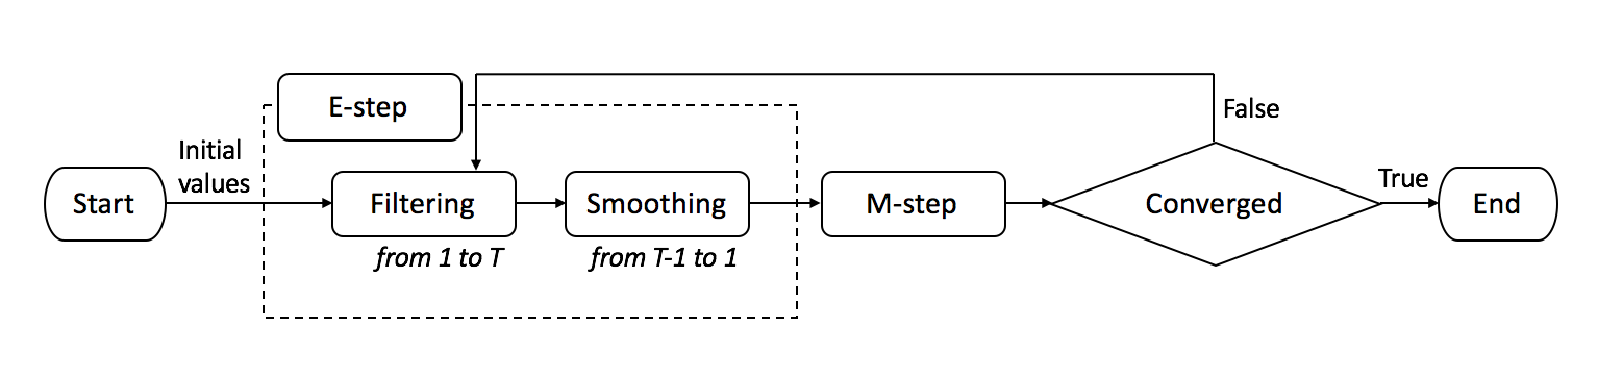
\includegraphics[scale=0.55]{picture/em}
\par\end{centering}
\caption{A flowchart showing the process of the Expectation-Maximization algorithm.
The algorithm begins with a set of initial values. The E-step is performed
by computing a filtering and smoothing algorithm. Then, the M-step
is performed. Iterating both steps until convergence.}

\label{em}
\end{figure}


\subsubsection{E-step}

In this step, $\theta^{(n)}$ is the derived set of parameters in
M-step from the previous iteration, and $n$ is a current iteration
in the algorithm. The available observations of time $t-1$ is denoted
as $\Omega_{t-1}=(y_{1},y_{2},...,y_{t-1})$. The general idea of
this step is to calculate the expectation of $S_{t}$ under the current
estimation of the parameters. The obtained result is called smoothed
inferences probability, and is denoted by $P(S_{t}=j|\Omega_{T};\theta)$
where $T$ is the number of all observations in the data and $j=1,2,...,k$.
The E-step which consists of filtering and smoothing algorithm is
described as follows \citep{kim1994dynamic}:

\paragraph{Filtering}

A filtered probability is a probability of a non-observable Markov
chain being in a given state $j$ at time $t$, conditional on information
up to time $t$. The algorithm starts from $t=1$ to $t=T$. A starting
point for the first iteration where $t=1$ is chosen from arbitrary
values. The probabilities of each state given available observations
up to time $t-1$ is calculated by

\begin{equation}
P(S_{t}=j|\Omega_{t-1};\theta^{(n)})=\sum_{i=1}^{k}p_{ij}^{(n)}P(S_{t-1}=i|\Omega_{t-1};\theta^{(n)})\qquad j=1,2,...,k
\end{equation}

The conditional densities of $y_{t}$ given $\Omega_{t-1}$ are

\begin{equation}
f(y_{t}|\Omega_{t-1};\theta^{(n)})=\sum_{j=1}^{k}f(y_{t}|S_{t}=j,\Omega_{t-1};\theta^{(n)})P(S_{t}=j|\Omega_{t-1};\theta^{(n)})
\end{equation}

where $f(y_{t}|S_{t},\Omega_{t-1};\theta)=\frac{1}{\sqrt{2\pi\sigma_{S_{t}}^{2}}}exp\left\{ -\frac{(y_{t}-\beta_{S_{t}})^{2}}{2\sigma_{S_{t}}^{2}}\right\} $
is the likelihood function in each state for time $t$. This is simply
a Gaussian probability density function.

Then, with the new observation at time $t$, the probabilities of
each state are updated by using Bayes' rule as shown below

\begin{equation}
P(S_{t}=j|\Omega_{t};\theta^{(n)})=\frac{f(y_{t}|S_{t}=j,\Omega_{t-1};\theta^{(n)})P(S_{t}=j|\Omega_{t-1};\theta^{(n)})}{f(y_{t}|\Omega_{t-1};\theta^{(n)})}\label{eq:fProb}
\end{equation}

The process above is computed iteratively until all the observation
is reached i.e., $t=T$.

\begin{comment}
The joint conditional density function of $y_{t},$$S_{t-1}$and $S_{t}$
given $\Omega_{\ensuremath{t-1}}$ are

\[
f(y_{t},S_{t-1}=i,S_{t}=j|\Omega_{t-1};\theta^{(n)})=f(y_{t}|S_{t-1}=i,S_{t=}j,\Omega_{t-1};\theta^{(n)})P(S_{t-1}=i,S_{t}=j|\Omega_{t-1};\theta^{(n)})
\]

and 

\[
P(S_{t-1}=i,S_{t}=j|\Omega_{t};\theta^{(n)})=\frac{f(y_{t},S_{t-1}=i,S_{t}=j|\Omega_{t-1};\theta^{(n)})}{f(y_{t}|\Omega_{t-1};\theta^{(n)})}
\]
\end{comment}


\paragraph{Smoothing}

A smoothed probability is a probability of a non-observable Markov
chain being in state $j$ at time $t$, conditional on all available
information. The algorithm iterates over $t=T-1,T-2,...,1$. The starting
values are obtained from the final iteration of the filtered probabilities.

By noting that

\begin{align}
P(S_{t}=j|S_{t+1}=i,\Omega_{T};\theta^{(n)}) & \thickapprox P(S_{t}=j|S_{t+1}=i,\Omega_{t};\theta^{(n)})\nonumber \\
 & =\frac{P(S_{t}=j,S_{t+1}=i|\Omega_{t};\theta^{(n)})}{P(S_{t+1}=i|\Omega_{t};\theta^{(n)})}\nonumber \\
 & =\frac{P(S_{t}=j|\Omega_{t};\theta^{(n)})p_{ij}^{(n)}}{P(S_{t+1}=i|\Omega_{t};\theta^{(n)})}
\end{align}

and

\begin{equation}
P(S_{t}=j|\Omega_{T};\theta^{(n)})=\sum_{i=1}^{k}P(S_{t}=j,S_{t+1}=i|\Omega_{T};\theta^{(n)})
\end{equation}

then, the smoothed probabilities can be expressed as

\begin{equation}
P(S_{t}=j|\Omega_{T};\theta^{(n)})=\sum_{i=1}^{k}\frac{P(S_{t+1}=i|\Omega_{T};\theta^{(n)})P(S_{t}=j|\Omega_{t};\theta^{(n)})p_{ij}^{(n)}}{P(S_{t+1}=i|\Omega_{t};\theta^{(n)})}
\end{equation}


\paragraph{Full log-likelihood}

Once the filtered probabilities are estimated, there is enough necessary
information to compute the full log-likelihood function.

\begin{equation}
\ln L(\theta)=\sum_{t=1}^{T}\ln(f(y_{t}|\Omega_{t-1};\theta^{(n)})=\sum_{t=1}^{T}\ln\sum_{j=1}^{k}((f(y_{t}|S_{t}=j,\Omega_{t-1};\theta^{(n)})P(S_{t}=j|\Omega_{t-1}))\label{eq:loglik}
\end{equation}

This is simply a weighted average of the likelihood function in each
state. The probabilities of states are considered as weights.

\subsubsection{M-step}

The new estimated model parameters $\theta^{(n+1)}$ are obtained
by finding a set of parameters that maximizes Equation \ref{eq:loglik}.
This new set of parameters is more precise and better than the previous
estimated value of the maximum likelihood. $\theta^{(n+1)}$ serves
as a set of parameters in the next iteration of the E-step. 

Each individual parameter in $\theta^{(n+1)}$ are taken from its
maximum value, which is determined by taking partial derivative of
the log-likelihood function with respect to each parameter. Generally,
this process is similar to the standard maximum likelihood estimation.
However, it has to be weighted by the smoothed probabilities because
each observation $y_{t}$ contains probability from each $k$ states.
\begin{comment}
any of the $k$ states
\end{comment}


\subsubsection{Convergence of the E-M algorithm}

The E- and M-step are iteratively computed until the algorithm converges.
The algorithm will terminate when the different between the previous
and current estimate values is less than a specific value. This specific
value called a stopping criteria needs to be specified beforehand.
The convergence is assured since the value of the log-likelihood function
will increase in each iteration. However, the E-M algorithm does not
guarantee to always converge to a global maximum. The convergence
of the algorithm is also possible to be only a local maxima. %
\begin{comment}
It is possible for the algorithm to converge to local maxima
\end{comment}

\begin{comment}
(max(abs(object{[}\textquotedbl{}Fit\textquotedbl{}{]}{[}\textquotedbl{}logLikel\textquotedbl{}{]}
- oldll))/(0.1 + max(abs(object{[}\textquotedbl{}Fit\textquotedbl{}{]}{[}\textquotedbl{}logLikel\textquotedbl{}{]})))
< control\$tol)

\&

(max(abs(object{[}\textquotedbl{}Coef\textquotedbl{}{]}-oldcoef),na.rm=TRUE)/(0.1+max(abs(object{[}\textquotedbl{}Coef\textquotedbl{}{]}),na.rm=TRUE))
< control\$tol) )
\end{comment}


\section{State prediction}

A function to predict the most probable state for the new observation
is implemented in \emph{R} as an additional function in the package
for this analysis (see \ref{sec:MSwM-Package}).

The probabilities of being in state $j$ at time $T+1$ on a basis
of the current information are computed by performing the filtering
algorithm in the E-step of E-M algorithm. The filtered probabilities
are

\[
P(S_{T+1}=j|\Omega_{T+1};\theta)=\frac{f(y_{T+1}|S_{T+1}=j,\Omega_{T};\theta)P(S_{T+1}=j|\Omega_{T};\theta)}{f(y_{T+1}|\Omega_{T};\theta)}
\]

This is Equation \ref{eq:fProb} where $t=T+1$. Then, the new observation
at time $T+1$ is said to be in the state $j$ if it has the highest
probability.

\section{Model selection}

In this study, several Markov switching models will be carried out.
First, the number of states $k$ for the model will be chosen. Then,
the number of switching coefficients in the model will be decided.
Models will be selected based on the quality of the model. 

Model selection is a task of selecting the best model for a given
set of data. The Bayesian Information Criterion (BIC) is widely employed
in the applied literature, and proved to be useful in selecting the
model among a finite set of models (e.g., \citet{leroux1992maximum}
used BIC to select the number of states $k$). It is also known as
Schwarz Information Criterion \citep{schwarz1978estimating}. Model
which has a lower value of BIC is preferred. 

\[
\mathrm{BIC}=-2\ln(L(\hat{\theta}))+m\cdot\ln(T)
\]

where $L(\hat{\theta})$ represents the maximized value of the likelihood
function, $T$ is the number of observations, and $m$ is the number
of parameters to be estimated in the model. While including more parameters
or terms will result in a higher likelihood, it can also leads to
an overfitting. BIC attempts to reduce the risk of overfitting by
taking into account the number of parameters in the model. BIC can,
therefore, heavily penalizes a model complexity. %
\begin{comment}
One benefit from using BIC is that this criterion heavily penalizes
model complexity as it takes into account the number of parameters
in the model. In addition, BIC attempts to reduce the risk of overfitting.
\end{comment}


\section{Non-parametric analysis}

A parametric analysis outperform a non-parametric analysis if the
applied data belongs to a known distribution family. However, a parametric
test does not perform well in detecting change point of an unknown
underlying distribution \citep{sharkey2014nonparametric}. Applying
a non-parametric analysis to a real-world process gives a real advantage
to the analysis. Data collected from a real-world process, in general,
usually does not have a well-defined structure, which is more suitable
to be applied with the non-parametric analysis that is not too restricted
\citep{hawkins2010nonparametric}. For this reason, the non-parametric
analysis is implemented in order to get a rough idea of the change
point location in this thesis framework. The obtained result is also
compared with the result from using the Markov switching autoregressive
model.

\subsubsection*{E-divisive}

An \emph{ecp}\footnote{https://cran.r-project.org/web/packages/ecp/index.html}
is an extension package in \emph{R} which mainly focuses on computing
a non-parametric test for multiple change point analysis. This change
point method is applicable to both univariate and multivariate time
series. A fundamental idea of the package is based on the hierarchical
clustering approach \citep{james2013ecp}. 

An E-divisive method is an algorithm in the \emph{ecp} package. This
algorithm performs a divisive clustering in order to estimate the
multiple change points. The E-divisive recursively partitions a time
series and estimates a single change point in each iteration. Consequently,
the new change point is located in each iteration, which divides the
time series into different segments. The algorithm also uses a permutation
test to compute the statistical significance of an estimated change
point. More details about the estimation is described in \citet{matteson2014nonparametric}.
The computational time of the E-divisive algorithm is $O(kT^{2})$,
where $k$ is number of estimated change points and $T$ is number
of observations in the time series data.

\begin{comment}
E-agglomerative

The E-agglomerative algorithm performs an agglomerative clustering
in favor of estimating the multiple change points. The algorithm tries
to maximize a goodness of fit test after merging segments in the iteration.
The estimated change point is defined by the iteration that maximized
a goodness of fit statistic. This algorithm allows users to input
an initial segmentation for the time series or a prior knowledge of
the possible change point in order to reduce the computation time. 
\end{comment}


\section{Simulation study}

The state of the CPU in a real data is unknown in the study. As a
consequence, an accuracy of the Markov switching model and the E-divisive
method cannot be computed, and the comparison between both methods
can hardly make. One possible solution to test how effective both
methods are, and to verify how well the implemented state prediction
function performs is to used a simulation technique. The dataset that
consists of two predictor variables and one response variable with
already known states is simulated. The actual models of each state
are 

\[
y_{t}=\begin{cases}
\begin{array}{c}
10+0.6X_{1,t}-0.9X{}_{2,t}+0.5y_{t-1}+\varepsilon_{t}^{(1)}\\
2+0.8X_{1,t}+0.2y_{t-1}+\varepsilon_{t}^{(2)}\\
-12+0.7X_{1,t}+0.2X{}_{2.t}-0.2y_{t-1}+\varepsilon_{t}^{(3)}
\end{array} & \begin{array}{c}
\varepsilon_{t}^{(1)}\sim N(0,1);\quad\mathrm{Normal}\\
\varepsilon_{t}^{(2)}\sim N(2,0.5);\quad\mathrm{Bad}\\
\varepsilon_{t}^{(3)}\sim N(1,1);\quad\mathrm{Good}
\end{array}\end{cases}
\]

where, 
\begin{labeling}{00.00.0000}
\item [{$y_{t}$}] is assumed to be a value of a CPU usage of the time
series at time $t$
\item [{$x_{1,t}$}] is a predictor variable generated by a uniform distribution
on $[50,200]$ of the time series at time $t$
\item [{$x_{2,t}$}] is a predictor variable generated by a uniform distribution
on $[0,50]$ of the time series at time $t$
\end{labeling}
There are two simulated datasets \textendash{} Dataset 1 and Dataset
2 \textendash{} and each of them contains 500 observations. Both datasets
have different time periods where the switches between states occur.
The simulated Dataset 1 has a longer duration to remain in its own
state before switching to the other states than the simulated Dataset
2. \ref{sim_data} and \ref{sim_data2} present plots of $y$ over
a period of time, and the period where observations in the data belong
to one of the state for the first and second simulated data, respectively.

\begin{comment}
The simulated data contains 500 observations. \ref{sim_data} presents
a plot of $y$ over a period of time, and the period where observations
in the data belong to one of the state.
\end{comment}

\begin{comment}
The simulated data, which contains 500 observations, has three different
states \textendash{} Normal, Bad and Good. 
\end{comment}

\begin{figure}[H]
\begin{centering}
\includegraphics[scale=0.35]{picture/sim1}
\par\end{centering}
\caption{\emph{Top:} A simulated data of Dataset 1 where $y$ variable is the
response variable. \emph{Bottom:} The period in the time series when
observation is in each state.}
\label{sim_data}
\end{figure}

\begin{figure}[H]
\begin{centering}
\includegraphics[scale=0.35]{picture/sim2}
\par\end{centering}
\caption{\emph{Top:} A simulated data of Dataset 2 where $y$ variable is the
response variable. \emph{Bottom:} The period in the time series when
observation is in each state.}
\label{sim_data2}
\end{figure}


\section{Technical aspects}

The thesis work has been carried out using the \emph{R} programming
language for the purpose of data cleaning, preprocessing, and analysis.
The Markov switching model was performed using the \emph{MSwM} package.
Various extensions and modifications were implemented in the package
(see \ref{sec:MSwM-Package}). For the E-divisive method, the \emph{ecp}
package was used. 


